\documentclass[11pt]{scrartcl}
\usepackage[utf8]{inputenc} % Kodierung der Textdatei mit Sonderzeichen
\usepackage[ngerman]{babel} % Sprache für Inhaltsverzeichnis etc.
\usepackage{amssymb} % Mathematische Symbole
\usepackage{amsmath} % Mehr mathematische Konstrukte
\usepackage{graphicx} % Um Bilder einbinden zu können
\usepackage{float} % für \begin{figure}[H]



\newcommand{\unit}[1]{\ensuremath{\,\mathrm{#1}}} % Einheiten schreiben sich immer aufrecht!
\newcommand{\degr}{\ensuremath{^\circ}}
\newcommand{\cel}{\ensuremath{\degr\mathrm{C}}}
\newcommand{\dif}{\ensuremath{\mathrm{d}}}
\newcommand{\pdif}[2]{\ensuremath{\frac{\partial#1}{\partial#2}}}
\newcommand{\ee}[1]{\ensuremath{\cdot 10^{#1}}}



\title{Gr\"atzelzelle - Gruppe 5 WS 09/10, Projektpraktikum der Uni Erlangen}
\date{19.10.2009 -- 31.10.2009}
\author{Michele Collodo, Andreas Glossner, Karl-Christoph Gödel, Bastian Hacker, Maria Obst, Alexander Wagner, David Winnekens}



\begin{document}
\sloppy % lässt Latex nicht über den Rand rausschreiben
\thispagestyle{empty}
\large{Projektpraktikum WS 09/10}
\hfill
\raisebox{-1.4cm}{
\includegraphics[width=5cm]{images/fau.pdf}}
\\[8\baselineskip]
\begin{center}
{\Huge\textbf{Gr\"atzelzelle}}
\\[0.5\baselineskip]
{\large Energieforschung auf der Nanoebene}
\\[1.5\baselineskip]
{\Large 19.10.2009 -- 31.10.2009}
\\[6\baselineskip]
{\Huge\textbf{PPG 5}}\\[0.5\baselineskip]
{\large\textbf{
Michele Collodo,
Andreas Glossner,\\
Karl-Christoph Gödel,
Bastian Hacker,\\
Maria Obst,
Alexander Wagner,
David Winnekens}\\
Tutor: Xiaoyue Jin}
\vfill



\small{\texttt{http://pp.physik.uni-erlangen.de/groups/ws0910/ppg5/ppg5\_start.html}}
\end{center}
\newpage



\tableofcontents
\vfill



\begin{abstract}
%%% Maria

Description of our work \ldots
\end{abstract}
\newpage



\section{Einleitung}
relativ kurz \ldots
\section{Theorie}
\subsection{B\"andermodell und Halbleitertechnik}
Um die Funktionsweise von Solarzellen im allgemeinen und der Gr\"atzelzelle im besonderen verstehen zu k\"onnen, muss man sich zun\"achst mit dem Energieb\"andermodell aus der Quantenmechanik besch\"aftigen. Die B\"ander entstehen durch \"Uberlagerung der Energieniveaus der einzelnen, im Kristall dicht nebeneinander gelagerten Atome. Nahe bei den Atomr\"umpfen befinden sich die gebundenen Zust\"ande. Wenig dar\"uber entsteht durch \"Uberlappung der Potentiale das Valenzband, in dem alle Pl\"atze mit Elektronen besetzt sind. So kann sich ein Elektron nur bewegen, wenn sich ein andres Elektron genau in entgegengesetzter Richtung bewegt. 
Noch weiter von den Atomr\"umpfen entfernt liegen weitere, unbesetzte Energieniveaeus \"ubereinander. Hier k\"onnen sich die Elektronen frei bewegen, dieses Band wird daher Leitungsband genannt.\newline
Zwischen Valenz- und Leitungsband befindet sich die verbotene Zone (Bandl\"ucke), in der sich keine Elektronen befinden. Nach der Gr\"o\ss{}e dieser Zone unterscheidet man Leiter, Halbleiter und Isolatoren. Bei einem Leiter gibt es keine verbotene Zone und Valenz- und Leitungsband gehen ineinander \"uber oder im Valenzband sind nicht alle Pl\"atze mit Elektronen besetzt. So kann problemlos Strom fliessen. Isolatoren hingegen haben ein vollst\"andig besetztes Valenzband und die Bandl\"ucke ist so gro\ss{} dass sie selbst von hoch angeregten Elektronen nicht oder nur sehr schwer \"uberwunden werden kann.\newline
Auch bei Halbleitern ist das Valenzband voll besetzt, jedoch ist hier die verbotene Zone noch kleiner als etwa 10eV. Es ist also f\"ur Elektronen, die durch hohe Temperaturen oder einfallende Photonen angeregt sind, m\"oglich, die L\"ucke zu \"uberspringen und sich im Leitungsband fortzubewegen. Werden hier nun in den Kristall Fremdatome eingef\"ugt (Dotierung), ver\"andern sich dessen leitenden Eigenschaften. Werden Atome eingesetzt, die mehr Elektronen in der \"au\ss{}eren Schale haben als die des Kristalls (n-Dotierung), so gibt es \glqq\"ubersch\"ussige\grqq Elektronen, die einfacher ins Leitungsband wechseln k\"onnen. Solche Atome hei\ss{}en Elektronendonatoren. F\"ugt man hingegen Fremdatome ein, die weniger Elektronen in ihrer \"au\ss{}eren Schale haben (p-Dotierung), entstehen L\"ocher, in denen leicht Elektronen aus dem Valenzband angelagert werden. Es gibt nun Elektronenfehlstellen, die Atome werden als Elektronenakzeptoren bezeichnet.\newline
Bringt man nun einen p-dotierten und einen n-dotierten Halbleiter zusammen, diffundieren die \"ubersch\"ussigen Elektronen aus der n-Schicht zu den Fehlstellen in der p-Schicht, es bildet sich ein elektrisches Feld, das von der n- zur p-Seite gerichtet ist. Nun k\"onnen durch das Anlegen einer \"au\ss{}eren Spannung verschiedene Funktionen, wie beispielsweise die Diode, erreicht werden. Schliesst man den Pluspol an die p-Schicht und den Minuspol an die n-Schicht, betreibt man eine Diode in Durchlassrichtung. Die Bandl\"ucke wird beinahe aufgehoben und Leitung ist m\"oglich.\newline
Bei umgekehrter Polung, also in Sperrichtung, kann kein Strom flie\ss{}en. Solche Dioden nennt man Photodioden, sie werden in herk\"ommlichen Solarzellen verwendet. Eine Gr\"atzelzelle hingegen greift mehr auf Ideen der Natur zur\"uck. Hier wird durch Imitation der nat\"urlichen Photosynthese Energie erzeugt.

\subsection{Funktionsweise der Gr\"atzelzelle}
Die Gr\"atzelzelle, benannt nach ihrem Erfinder, dem Schweizer Michael Gr\"atzel, besteht aus zwei Elektroden, typischerweise leitend beschichtete Glasplatten. Auf der einen Glasplatte wird als Halbleiter Titandioxid angebracht. Da hier aber die verbotene Zone aber eine Gr\"o\ss{}e von 3.2eV hat, w\"are die Zelle nur f\"ur hochenergetische Photonen des UV-Lichts empfindlich. Daher wird auf die TiO$_{2}$-Schicht ein lichtempfindlicher organischer Farbstoff aufgebracht, dessen Elektronen auch von sichtbarem Licht angeregt werden k\"onnen. Die Gr\"atzelzelle wird deshalb auch als Farbstoffsolarzelle bezeichnet.\newline
Die Gegenelektrode ist mit einem Katalysator, oft Platin, beschichtet, um die \"Ubergabe der ausgel\"osten Elektronen zu erleichtern. Den Raum zwischen den beiden Elektroden f\"ullt ein Elektrolyt, der in Redox-Reaktionen einerseits dem Farbstoff schnellen Nachschub an Elektronen liefert und andererseits an der Kathode wieder zur\"uck reagiert. Hier wird h\"aufig Iodkaliumiodid eingesetzt.

\section{Aufbau}
\subsection{Materialien, Beschaffung und Bau der Zelle}
%%% Karl
Die Beschaffung der f\"ur den Bau ben\"otigten Materialien stellte zu Beginn ein Problem dar. Insbesondere war es schwer, leitende und gleichzeitig transparente Elektroden zu bekommen. Die erste M\"oglichkeit, mit Gold beschichtet Glaspl\"attchen, zu verwenden, scheiterte an den zu geringen Ausma\ss{}en der m\"oglichen Tr\"agerplatten. Zu lange Lieferzeiten und zu hohe Prei\ss{}e schlossen auch die Bestellung von industriell produzierten ITO-Gl\"asern (Indiumzinnoxid-Beschichtung) aus.
Das Institut der Physikalischen Chemie der Universit\"at Erlangen stellte gl\"ucklicherweise mehrere Fluorzinnoxid (FTO) beschichtete Glasplatten zur Verf\"ugung. Die leitend beschichteten, transparenten Glasplatten waren bereits auf eine Gr\"o\ss{}e von \(70\unit{mm} \times 20\unit{mm} \times 4 \unit{mm}\) zugeschnitten. Auf der leitenden Seite der Glasplatte konnte mit Hilfe eines Multimeters ein Widerstand von etwa \(20 \frac{\unit{\Omega}}{\unit{cm}}\) gemessen werden.\newline
Das Elektrolyt, eine Iod-Kaliumiodid-L\"osung sowie verd\"unnte Salzs\"aure zum Anmischen der Titandioxidpaste konnten ebenfalls von der Physikalischen Chemie bezogen werden.
\subsection{Versuchsanordnung}
%%% Michele und Axi
\begin{figure}[ht]
\begin{center}
% Zeichnung mit xcircuit
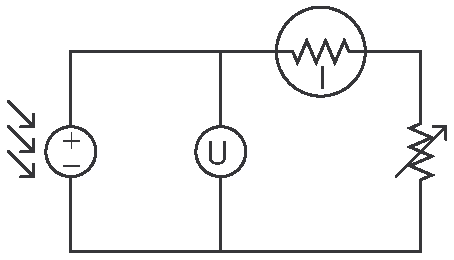
\includegraphics[width=0.8\textwidth]{images/leistungsmesskreis.pdf}
\end{center}
\vspace{-1.5\baselineskip}
\caption{Schaltkreis zur Leistungsmessung. Das Amperemeter hatte einen signifikaneten Eigenwiderstand.}
\label{leistungsschaltkreis}
\end{figure}
Schaltung (ltspice scheint nicht das richtige zu sein. Vielleicht doch mit Inkscape und großem gitter zeichnen. siehe auch http://en.wikipedia.org/wiki/Wikipedia:WikiProject\_Electronics/Programs !),
Geraete, ...
\section{Messungen und Ergebnisse}
%%% Basti, Michele (LED's)
\subsection{Leistung}
\subsection{Wellenl\"ange}
\section{Fazit}
%%% zusammen
Dank an Vito Wieauchimmer, etc.
\end{document}

